\documentclass{scrreprt} 
%scrreprt is a KOMAScript class
%KOMASCript Documentation https://komascript.de/~mkohm/scrguide.pdf

%according to screprt documentation include all options in the following command:
\KOMAoptions{
fontsize=11pt, 
paper=a4, 
abstract=true, 
listof=totoc, 
bibliography=totoc, 
numbers=noenddot}
% A4 paper is default in scrreprt class, abstract=true activates abstract section with headline
% listof = totoc -> makes lists appear in the toc
% bibliography=totoc -> add bibliography to toc 
%numbers=noenddot -> usually, when alphanumeric numbering is used, i.e. appendix, numbers end with dot (ISO 2145) -> this is to switch this off.
%consider KOMA script documentation on scrreprt http://babyname.tips/mirrors/ctan/macros/latex/contrib/koma-script/doc/scrguien.pdf

% please check submission procedure https://www.htwg-konstanz.de/master/informatik/studienorganisation/abschlussarbeit/

% include all files from settings folder
%load packages
% this file includes the packages that are used

\usepackage[colorinlistoftodos]{todonotes}
% begin todonotes package configuration
% documentation of todonotes package http://ctan.127001.ovh/macros/latex/contrib/todonotes/todonotes.pdf

% write todos inline instead of margin
%\presetkeys{todonotes}{inline}{}

% define todo commands for multiple purposes with different colors
% \todo = general todo
\newcommand{\todogen}[1]{\todo[inline]{#1}} %make general todo inline
\newcommand{\todoref}[1]{\todo[inline, color=yellow]{#1}} % check or add reference
\newcommand{\todoresearch}[1]{\todo[inline, color=violet]{#1}} % more research necessary
\newcommand{\tododetail}[1]{\todo[inline, color=cyan]{#1}} % more details please
\newcommand{\todolayout}[1]{\todo[inline, color=magenta]{#1}} % layout issue to be fixed
\newcommand{\todocheck}[1]{\todo[inline, color=teal]{#1}} % double check or verifiy
\newcommand{\todocorrect}[1]{\todo[inline, color=red]{#1}} % wrong statement, please correct
\newcommand{\todoreview}[1]{\todo[inline, color=blue]{#1}} % this section is ready for review

%end todonotes package configuration

% Only necessary when using official HTWG authorship declaration of authorship as PDF
%\usepackage{pdfpages}

\usepackage{listings} %to use source code
%begin listings configuration
\lstset{language=Python} %Python as default language 

%Think about changing name tag for listings...
%\renewcommand{\lstlistingname}{Algorithm}% Listing -> Algorithm
%\renewcommand{\lstlistlistingname}{List of \lstlistingname s}% List of Listings -> List of Algorithms
%ftp://ftp.fu-berlin.de/tex/CTAN/macros/latex/contrib/listings/listings.pdf
%https://en.wikibooks.org/wiki/LaTeX/Source_Code_Listings
%https://www.macwrench.de/wiki/Kurztipp_-_Quellcodelistings_in_LaTeX
%end listings configuration

%acronyms
\usepackage{acronym}

%add bibliography to toc
%\usepackage{tocbibind} -> can be defined in documentclass
%optional: change name Bibliography -> References https://tex.stackexchange.com/questions/12597/renaming-the-bibliography-page-using-bibtex
\renewcommand{\bibname}{References} 

%graphics
\usepackage{graphicx}



%last package is hyperref -> not necessary because bookmark includes hyperref!
%load hyperref package last to avoid conflicts, because it overrides some commands
%http://latex.hpfsc.de/content/latex_tipps_und_tricks/links_urls_pdf/
%\usepackage{hyperref}

%use hyperref instead of bookmark
%check hyperref package for linking
%bookmarks in PDF file
\usepackage[numbered]{bookmark}
%ftp://ftp.mpi-sb.mpg.de/pub/tex/mirror/ftp.dante.de/pub/tex/macros/latex/contrib/oberdiek/bookmark.pdf



%load customized layout
% this file contains all layout related settings
%load global variables
%this document defines the global variables, for multiple use within the document

%thesis title
\newcommand{\theTitle}{Fingerprint Presentation Attack Detection using Laser Speckle Contrast Imaging}

%supervisors
\newcommand{\supVis}{Prof. Dr. Hanno Langweg}
\newcommand{\supVisMail}{hanno.langweg@htwg-konstanz.de}
\newcommand{\supVisMailTo}{\href{mailto:\supVisMail}{\supVisMail}}
\newcommand{\coSup}{Jascha Kolberg, M.Sc.}
\newcommand{\coSupMail}{jascha.kolberg@h-da.de}
\newcommand{\coSupMailTo}{\href{mailto:\coSupMail}{\coSupMail}}

%dates
\newcommand{\submit}{June 30, 2018}

%author information
\newcommand{\theAuthor}{Pascal Keilbach}
\newcommand{\authorMail}{pascal.keilbach@htwg-konstanz.de}
\newcommand{\authorMailTo}{\href{mailto:\authorMail}{\authorMail}}
\newcommand{\matr}{294173}
\newcommand{\DoB}{17.07.1988}
\newcommand{\PoB}{Bad Mergentheim}

%cooperation
\newcommand{\coop}{Hochschule Darmstadt University of Applied Sciences, Biometrics and Internet-Security}

%htwg
\newcommand{\htwgAddress}{Hochschule Konstanz Technik, Wirtschaft und Gestaltung\\ University of Applied Sciences\\ Alfred-Wachtel-Stra{\ss}e 8\\ D-78462 Konstanz}
\newcommand{\dept}{Department of Computer Science}
%load titlepage setup
%this file includes the titlepage setup
%useful links
%https://de.wikibooks.org/wiki/LaTeX/_Eine_Titelseite_erstellen
%http://www.golatex.de/wiki/Schmutztitel
%KOMAScript Documentation chapter 3.7
%https://komascript.de/~mkohm/scrguide.pdf

%begin title page
\titlehead{
\includegraphics{img/htwgLogo} \hfill 
\includegraphics{img/htwgDept}}
\subject{Master Thesis}
\title{\theTitle}
\author{\theAuthor\\
	{\large\matr}\\ 
	{\large\authorMailTo}
}
\date{\submit}	
\subtitle{A thesis submitted in partial fulfillment of the requirements for the degree of Master of Science (M.Sc.)}
\publishers
{\small supervised by \vspace{3pt}\\ 
	{\large \supVis\thanks{\supVisMailTo}}\vspace{3pt}\\ 
	{\small and \vspace{3pt}}\\ 
	{\large \coSup\thanks{\coop, \coSupMailTo}}
}

%further options
%\extratitle{SCHMUTZTITEL} -> not necessary
%\dedication{If you want to change the world, start off by making your bed.}

%end title page



\begin{document}
%generate titlepage from information in settings/titlepage.tex file
\maketitle

%comment todos for final version
%this file contains the explanation of the todo items
\chapter*{Todo Legend}
\todogen{general todo}
\todoref{reference todo}
\todoresearch{research todo}
\tododetail{details...}
\todolayout{layout issue}
\todocheck{check again}
\todocorrect{correct this}
\todoreview{review}
\listoftodos

%start preface
\pagenumbering{roman}
% abstract

% guides on how to write an abstract: Google "How to write an abstract"
% http://phdtalk.blogspot.de/2011/08/how-to-write-abstract-in-30-minutes.html
% http://users.ece.cmu.edu/~koopman/essays/abstract.html
% https://writingcenter.unc.edu/tips-and-tools/abstracts/
% http://www.easterbrook.ca/steve/2010/01/how-to-write-a-scientific-abstract-in-six-easy-steps/
% http://hsp.berkeley.edu/sites/default/files/HOW%20TO%20WRITE%20AN%20ABSTRACT.pdf
% https://owl.english.purdue.edu/owl/resource/656/1/
\chapter*{Abstract}
%\begin{abstract}
\todolayout{Solution for uniform Headline}
This is the abstract.
\todogen{Write abstract, may consider guidelines}
Writing an abstract and conclusion is what you do at the very end of your thesis. 
Questions that might help to write a good abstract are:
	
	\begin{itemize}
		\item Motivation: Why do we care about the problem and the results?
		\item Problem statement: What problem are you trying to solve?
		\item Approach: How did you go about solving or making progress on the problem? Did you use simulation, analytic models, prototype construction, or analysis of field data for an actual product?
		\item Results: What's the answer?
		\item Conclusions: What are the implications of your answer? Is it going to change the world (unlikely), be a significant "win", be a nice hack, or simply serve as a road sign indicating that this path is a waste of time (all of the previous results are useful)? 		
	\end{itemize}

Do not itemize in final version.

	
%\end{abstract}
%declaration of authorship
%https://www.htwg-konstanz.de/master/informatik/studienorganisation/abschlussarbeit/
%sign on print version
%\addcontentsline{toc}{chapter}{Declaration of Authorship}
%Alternative Headings
%Declaration of Authorship
%Statement of Authorship
%Author's Declaration
%Declaration
\chapter*{Declaration of Authorship} %the * avoids numbering of heading
\textit{The official HTWG document is in German Language\footnote{\url{https://www.htwg-konstanz.de/fileadmin/pub/fk_in/Abschlussarbeiten/abschlussarbeiten_ehrenwoertliche_erklaerung_v2-170917.docx}}}
\newline
\newline
Hiermit erkläre ich, \theAuthor, geboren am \DoB\ in \PoB,
\newline
\newline
(1) dass ich meine Masterarbeit mit dem Titel:
\begin{center}
	\textbf{\theTitle}
\end{center}
am Institut da/sec unter Anleitung von \supVis\ selbständig und ohne fremde Hilfe angefertigt habe und keine anderen als die angeführten Hilfen benutzt habe;
\newline
\newline
(2) dass ich die Übernahme wörtlicher Zitate, von Tabellen, Zeichnungen, Bildern und Programmen aus der Literatur oder anderen Quellen (Internet) sowie die Verwendung der Gedanken anderer Autoren an den entsprechenden Stellen innerhalb der Arbeit gekennzeichnet habe.
\newline
\newline
(3) dass die eingereichten Abgabe-Exemplare in Papierform und im PDF-Format vollständig übereinstimmen.
\newline
\newline
Ich bin mir bewusst, dass eine falsche Erklärung rechtliche Folgen haben wird.
%fields for signature
\vspace{70pt}
\newline
Konstanz, den 30. Juni 2018
\newline

%\todolayout{Find better solution for Signature Lines}
\todolayout{Official English Version available? Mail to Prof. Mueller on 17.01.18}
\todolayout{If german Version must be used, check Umlaute!}

%alternative with signature lines
%\begin{tabular}{lp{2em}l}
%	\hspace{5cm}   && \hspace{5cm} \\\cline{1-1}\cline{3-3}
%	Ort, Datum     && Unterschrift
%\end{tabular}




%alternative: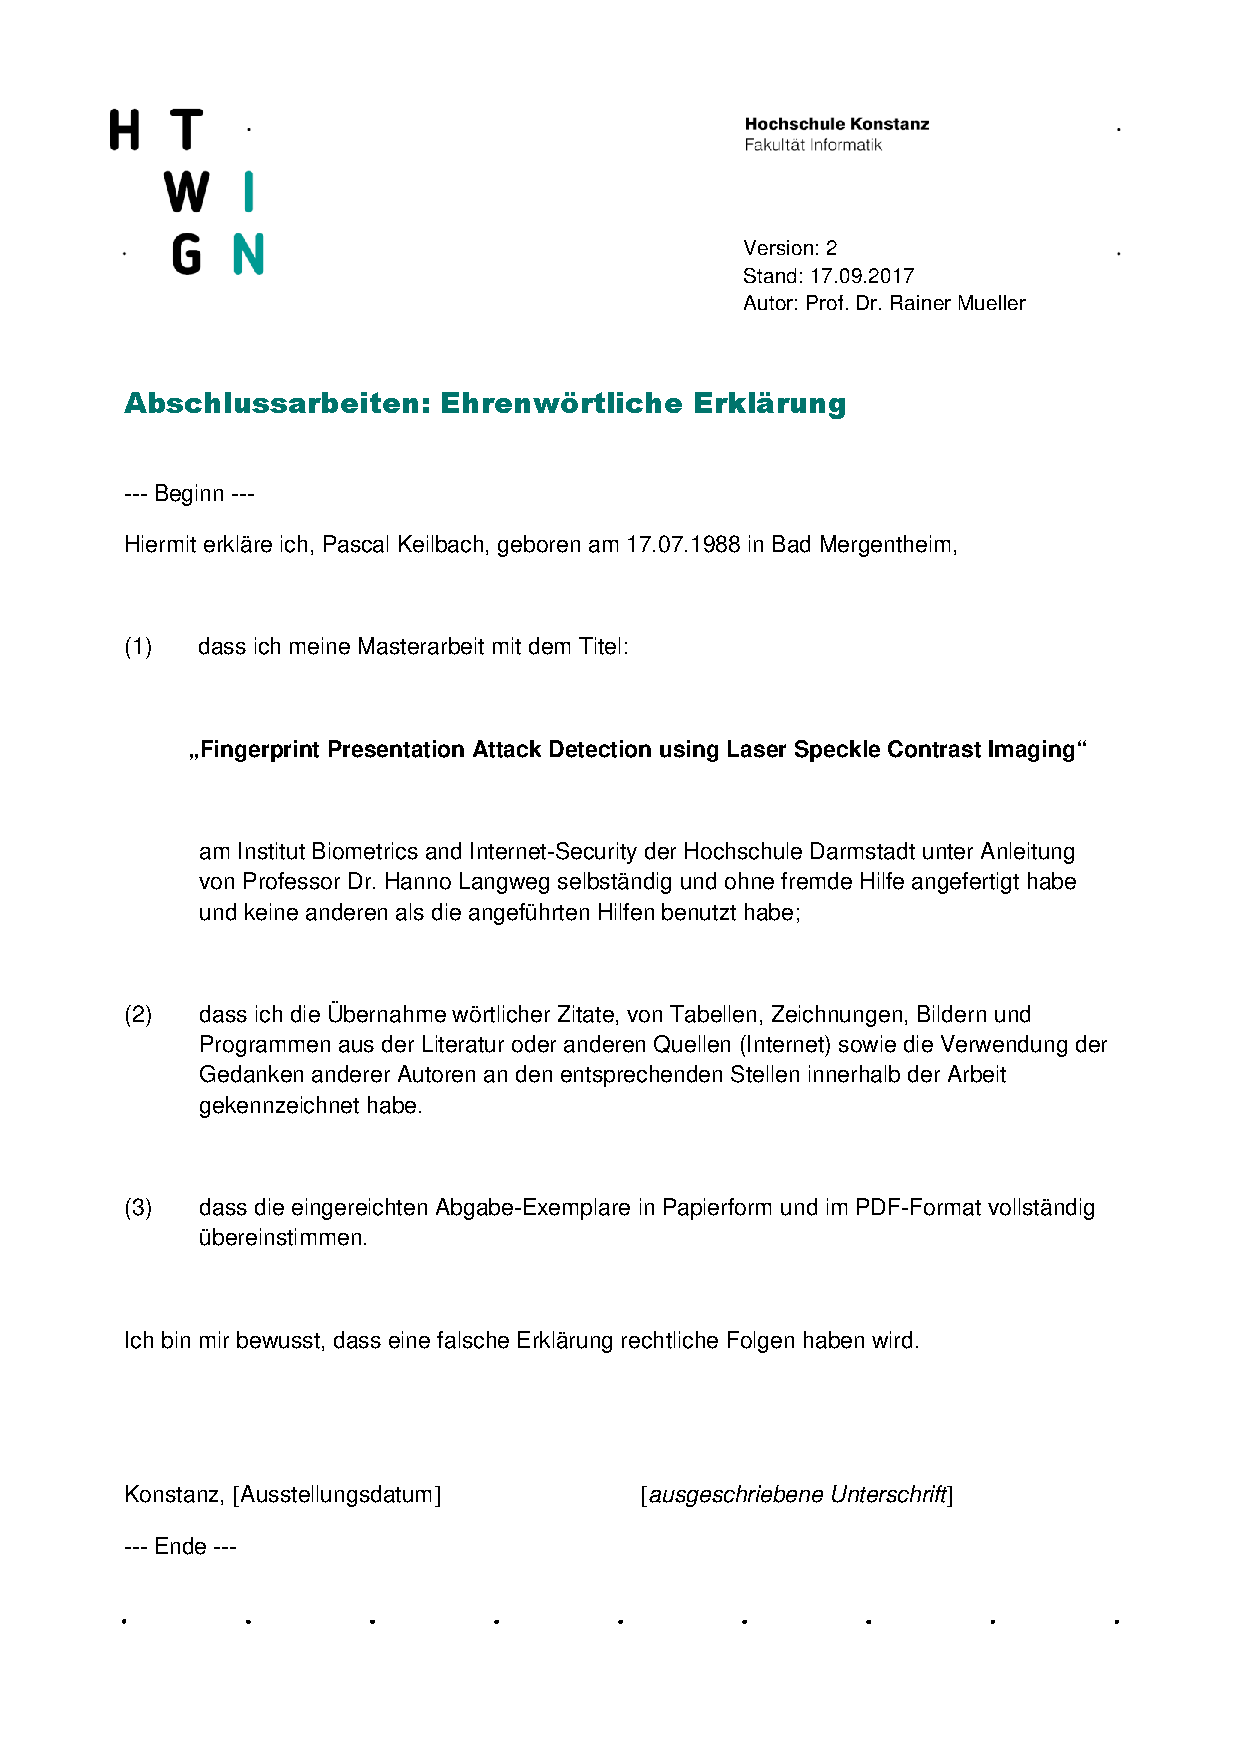
\includepdf[pages={1}]{preface/declaration.pdf}

%add pdfbookmark for toc
\pdfbookmark{\contentsname}{toc}
\tableofcontents
\todolayout{Think about Abstract and Author Declaration in TOC}

% lists of objects
\listoffigures
\listoftables
\lstlistoflistings
\todogen{Think about changing name for listings heading --> List of Listings}

%list of abbreviations
%this file contains all acronyms
%documentation:
%https://www.namsu.de/Extra/pakete/Acronym.html
%https://ctan.org/pkg/acronym?lang=de
\chapter*{List of Abbreviations}
 %add chapter to toc
\addcontentsline{toc}{chapter}{List of Abbreviations}
\begin{acronym}[LONGEST] %fit width of acronym column to longest acronym
	\acro{pad}[PAD]{Presentation Attack Detection}
	\acro{pa}[PA]{Presentation Attack}
	\acro{pai}[PAI]{Presentation Attack Instrument}
	\acro{eu}[EU]{European Union}
	\acro{long}[LONGEST]{The longest acronym in the list}
\end{acronym}



%end preface

% start content part of thesis
\pagenumbering{arabic}
\chapter{Introduction}\label{chap:01intro}
Test to use abbreviations \ac{pai}
this is a test quote \cite{EuropeanAssociationforBiometrics.2012}.
another test quote \cite{Busch.2014}
\chapter{Related Work}
\chapter{Data Analysis}
\chapter{Algorithm Implementation}
\chapter{Test Results}
\chapter{Evaluation}
\chapter{Conclusion and Future Work}
Conclusion

%end content part of thesis

%start references
%https://www.sharelatex.com/learn/Bibliography_management_with_bibtex#Bibliography_management_with_Bibtex
%\addcontentsline{toc}{chapter}{References}
\bibliography{bib/references}
\bibliographystyle{ieeetran} %http://www.ctan.org/pkg/ieeetran
\todolayout{Check citation style with hda}
%end references

%start appendix
%if appendix is used, a dot after numbering is done.
%use appendix only if necessary!
\appendix
%this file includes the appendices
\chapter{Appendix}
\section{First Appendix}
\section{Second Appendix}
%end appendix

\end{document}

%additional information
%compiling:
%http://www.bibtex.org/Using/

%order of chapters
%http://www.hrm.rub.de/studium/leitfaden/
%http://www.master-bachelor-korrektur.de/struktur.php
%http://www.holgermatthes.de/diplom-reader/gestaltung/formaler_aufbau.php
%referring to APA6 style
%https://tex.stackexchange.com/questions/88366/order-of-references-tables-figures-and-appendices-using-apa6-class
%http://guides.rasmussen.edu/apa/abstract-appendix
%http://www.apastyle.org/

